%!TEX root = ../thesis.tex

\section{Introduction}

Do it yourself (DIY) instructional videos show viewers how to carry
out physical tasks, such as craft projects, home improvement, repair,
or cooking~\cite{Torrey:2007he}. The availability of free
video-sharing sites like YouTube and Vimeo has led to an explosion in
user-generated video tutorials
online~\cite{Lafreniere:2012tl}. Effective instructional videos use a
range of video editing techniques, including subtitles, annotations, and
temporal speed up effects, to concisely communicate physical
procedures. However, producing high-quality videos requires
significant time investment and expertise. In addition to recording
possibly many takes, authors must review and cut the footage and then
apply the appropriate editing effects~\cite{Muller:2009tw}.
Instead of investing this effort, many amateurs instead create videos that simply show a long
uninterrupted recording of a demonstration.
%
While such videos are easy to produce, they often include a
lot of unnecessary footage (e.g., pauses, mistakes, long repetitive
actions) that makes it difficult for viewers to focus on the most
important steps and actions.
%
%\emph{Our research goal is to enable amateur users to produce
 % high-quality instructional videos while minimizing
 % post-demonstration editing}.

\begin{figure}[t]
  \centering
	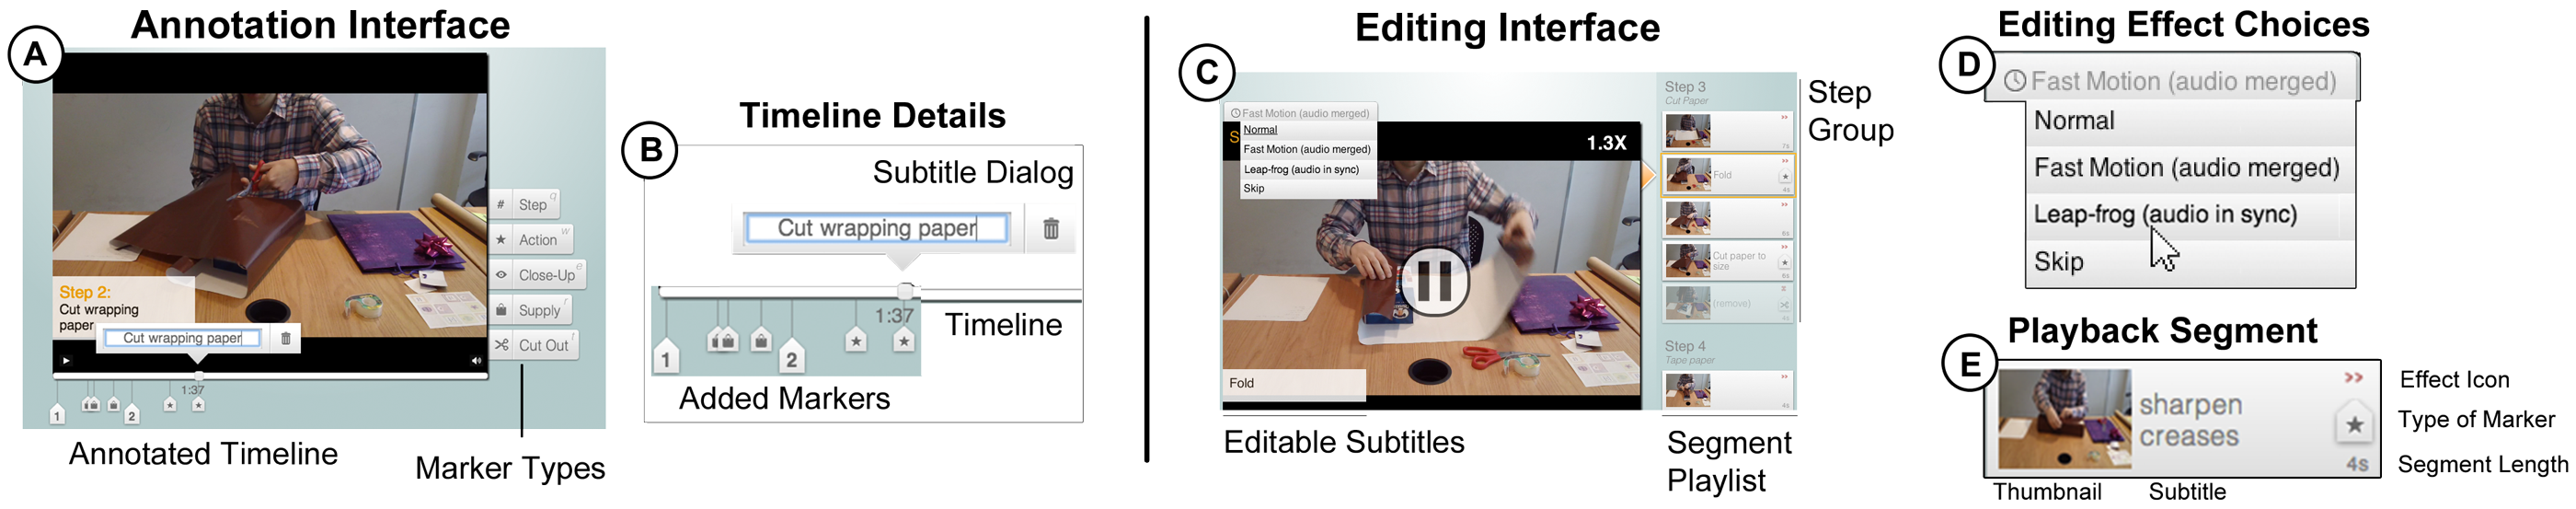
\includegraphics[width=\columnwidth]{\democut/fig/DemoCut}
  \caption{DemoCut automatically segments a single-shot demonstration recording and applies video editing effects based on user markers (A), including subtitles, fast motion (B), leap frog, zoom (C), and skip (D).}
  \label{fig:teaser}
\end{figure}

The goal of our work is to help amateur users produce effective instructional videos.
%
We analyzed existing DIY videos and interviewed video authors to uncover key challenges in creating high-quality
video tutorials: organizing long, single take recordings into
meaningful steps; removing/condensing unnecessary or repetitive
actions; and adding effects that emphasize important details in the
demonstration.
%
To address these challenges, we introduce DemoCut, a semi-automatic
video editing system that generates concise instructional videos from
recorded demonstrations (Figure~\ref{fig:teaser}).

With DemoCut, users record a single take of a narrated physical
task demonstration and then roughly annotate the recording with
markers that indicate high-level steps, important actions, supplies
and mistakes.
%
Based on these annotations, the system uses a combination of video and
audio analysis to automatically organize the recording into meaningful
segments and apply editing effects that make the tutorial more clear
and concise.
%
DemoCut supports both temporal effects that increase playback
speed or skip segments, as well as visual effects, such as
zooming, subtitles, and visual highlights.
%
DemoCut also provides an interface that allows users to quickly review
and edit the automatically generated effects.

We used DemoCut to create seven video tutorials in five
different DIY domains: electronics, crafts, art, repair and food.
The generated videos were concise in terms of video length and descriptive instructions with low effect error rates.
%\bh{Add some takeaway message of what we learned from this.}
%
We also conducted a small user study where participants used
our system to record and edit their own video tutorials.
%
All participants successfully created a complete tutorial that
included a variety of video editing effects, and the qualitative
feedback on DemoCut was very positive.
%
The participants felt that DemoCut enables a convenient workflow for
creating concise video tutorials and that the automatic editing
effects are particularly useful for speeding up repetitive
actions.

In summary, the main contributions of this work include:

\begin{itemize}
% \item A set of design implications for DIY video editing systems
%   derived from an analysis of existing video tutorials and interviews
%   with tutorial authors.
\item A light-weight annotation-based interface for editing instructional videos.
\item A set of marker types for annotation derived from our formative work. Markers represent different types of moments that lead to different editing effects.
\item A semi-automatic approach for editing DIY video that
  combines user annotation with audio and video analysis.
\item A working implementation of this approach and a preliminary evaluation with both novice and expert video editors.
\end{itemize}
